%!TEX root = ./presentation.tex 
\scrollmode

\documentclass[aspectratio=169]{beamer}
\usetheme{Madrid}


% -------------- COMPILE VARIABLES --------------
\newif\ifINTRO

\INTROfalse      % Build only intro slide


% ------------------ VARIABLES ------------------
\newcommand{\userName}{Pascal-Emmanuel Lachance}
\newcommand{\projectName}{PPPPP04}
\newcommand{\institution}{C3i}
\newcommand{\repo}{PPPPP}
\newcommand{\user}{raesangur}
\newcommand{\docName}{Presentation}

\author{\userName}
\title{\projectName}
\subtitle{Bonnes pratiques de design}
\institute{Compétitions de Conception de Circuits Imprimés}
\date{\today}


% ----------- CONFIGURATION INCLUDES ------------
%!TEX root = ../presentation.tex

%%%%%%%%%%%%
% PACKAGES %
%%%%%%%%%%%%

% =============== General Formatting ============
\usepackage[T1]{fontenc}
\usepackage{lmodern}
\usepackage{pifont}
\usepackage{amsmath}
\usepackage{amssymb}
\usepackage{fontawesome5}
\usepackage{comment}
\usepackage{adjustbox}
\usepackage{array}
\usepackage{multicol}
\usepackage[yyyymmdd]{datetime}

% =============== Colors ============
\usepackage{colortbl}
\usepackage[many]{tcolorbox}
\usepackage{xcolor}
\usepackage{hyperref}

% =============== Math ============
\usepackage{mathtools}
\usepackage{nicefrac}
\usepackage{siunitx}
\usepackage{calc}

% =============== Figures ============
\usepackage{tikz}
\usepackage{circuitikz}
\usepackage{pgfplots}
\usepackage{animate}
\usepackage{environ}

% =============== Listings ============
\tcbuselibrary{listings}      % Raesangur
\usepackage{listings}         % Main package for inserting code
\tcbset{listing engine={listings}}
\usepackage[scaled]{beramono} % For using the beramono font


% =============== Bibliography ============
%\usepackage{cite}

\usepackage[style=alphabetic,backend=biber, style=numeric, sorting=none]{biblatex}
%\addbibresource{references.bib}
\renewcommand*{\mkbibacro}[1]{#1}




% =============== Package Setup ============
\newcolumntype{C}[1]{>{\centering\arraybackslash}p{#1}}

\renewcommand{\dateseparator}{--}

\newcommand{\cmark}{\ding{51}} % ✓
\newcommand{\xmark}{\ding{55}} % ✗


% ------ Tikz ------
\usetikzlibrary{arrows, shapes, calc, positioning}
%\usetikzlibrary{external}
%\usepgfplotslibrary{external}
%\tikzexternalize
\pgfplotsset{compat=1.18}
%!TEX root = ../presentation.tex


% -------------- BACKGROUNDS --------------

\newcommand\titlebackground {
    \usebackgroundtemplate{
    \begin{tikzpicture}[remember picture, overlay]
        \node[at=(current page.center)] {
            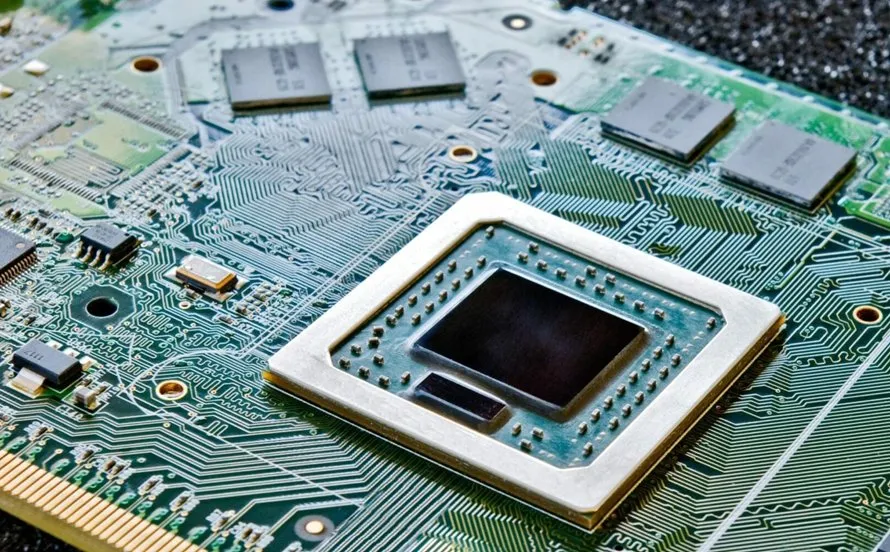
\includegraphics
            [width=\paperwidth, keepaspectratio]
            {pictures/background/background-PCB.png}
        };
    \end{tikzpicture}
    }
}


\newcommand\introbackground {
    \usebackgroundtemplate{
    \begin{tikzpicture}[remember picture, overlay]
        \node[at=(current page.center)] {
            
\includegraphics
            [width=\paperwidth, keepaspectratio]
            {pictures/background/background-pcb-poster.png}
        };
    \end{tikzpicture}
    }
}

\newcommand\defaultbackground {
    \usebackgroundtemplate{
    \begin{tikzpicture}[remember picture, overlay]
        \node[at=(current page.center)] {
            
\includegraphics
            [width=\paperwidth, keepaspectratio]
            {pictures/background/background5.pdf}
        };
    \end{tikzpicture}
    }
}


% -------------- TITLE PAGE --------------
\makeatletter
\setbeamertemplate{title page}
{
    \begin{columns}
        \begin{column}{0.75\textwidth}
            {
                
\includegraphics[scale = 0.35]{pictures/logo/udes_logo.pdf}\\
            }
            \vspace{24pt}
            \begin{tikzpicture}
                \def\boxwidth{\textwidth}
                \def\boxheight{3cm}
                \def\cornerradius{6pt}
                \def\shadowshift{0.5ex}
                
                \node[fill=UDSgreenSolidarite,
                      fill opacity=0.9,
                      rounded corners=6pt,
                      minimum width=\boxwidth, minimum height=\boxheight,
                      text=white,
                      text opacity=1,
                      align=center] (mainbox) at (0, 0){
                    \usebeamerfont{title}
                    \textbf{\inserttitle}\\
                    \usebeamerfont{subtitle}\usebeamercolor[fg]{subtitle}
                    \textbf{\insertsubtitle}\\\\
                    \small\usebeamerfont{author}\insertauthor
                };

                \path (mainbox) node[rectangle, minimum width=0.999\boxwidth, minimum height=0.996*\boxheight, rounded corners=\cornerradius, save path=\inbox] at (0, 0) {};
                \tikzset{protect=\inbox}

                \begin{scope}[transparency group, opacity=1]
                    \fill[color=black, opacity=0.33, rounded corners=\cornerradius,
                          blur shadow = {shadow xshift=.25ex, shadow yshift=-.25ex}]
                        (-0.5\boxwidth + \shadowshift, 0.5*\boxheight - \shadowshift) rectangle 
                        (0.5\boxwidth + \shadowshift, -0.5*\boxheight - \shadowshift);
                \end{scope}
            \end{tikzpicture}
            \vspace{24pt}
        \end{column}
        \begin{column}{0.25\textwidth}
        \end{column}
    \end{columns}
}
\makeatother


\newcommand\thankyouframe{
    \begin{frame}
    \begin{multicols}{2}
        \begin{beamercolorbox}[sep=8pt, center, shadow=true, rounded=true, wd=0.5\textwidth, bgopacity=0.85]{title}
            \usebeamerfont{title}Merci!\\
        \end{beamercolorbox}%
    \vfill\null
    \columnbreak
    \end{multicols}
\end{frame}
}

%!TEX root = ../presentation.tex



% Insert a figure with optional scaling and caption.
% 1: Width as a fraction of \textwidth   (default: 1)
% 2: Height as a fraction of \textheight (default: 0.8)
% 3: Caption text (optional)
% 4: Filename of the image (relative to 'pictures/' directory, no extension needed)
%
% Example:
% \makefigure[0.9][0.5][A sample image]{example-image}
\NewDocumentCommand{\makefigure}{O{1} O{0.8} o m}{%
    \begin{figure}%
        \centering%
        \includegraphics%
            [width=#1\textwidth, height=#2\textheight, keepaspectratio, page=1]%
            {pictures/#4}%
        \IfValueTF{#3}{%
            \caption*{#3}%
        }{}%
    \end{figure}%
}


% Insert a figure with border and with optional scaling and caption.
% 1: Width as a fraction of \textwidth   (default: 1)
% 2: Height as a fraction of \textheight (default: 0.8)
% 3: Caption text (optional)
% 4: Filename of the image (relative to 'pictures/' directory, no extension needed)
%
% Example:
% \makefigureborder[0.75][0.7][A sample image]{example-image}
\NewDocumentCommand{\makefigureborder}{O{1} O{0.8} o m}{%
    \begin{figure}%
        \centering%
        \tcbox[colframe=accent, colback=background]{
            \includegraphics%
                [width=#1\textwidth, height=#2\textheight, keepaspectratio, page=1]%
                {pictures/#4}%
            \IfValueTF{#3}{%
                \caption*{#3}%
            }{}%
        }
    \end{figure}%
}


% Create a TikZ circuit figure with adjustable size.
% 1: Width as a fraction of \textwidth   (default: 1)
% 2: Height as a fraction of \textheight (default: 0.8)
%
% Example:
% \begin{maketikzfigure}[0.7][0.5]
%     \draw (0,0) to[battery] (0,2);
% \end{maketikzfigure}
\NewDocumentEnvironment{maketikzfigure}{O{1} O{0.8}}{%
    \vspace{-16pt}%
    \begin{center}%
        \begin{adjustbox}{width=#1\textwidth, height=#2\textheight, keepaspectratio}%
            \begin{circuitikz}[american voltages]%
}
{%
            \end{circuitikz}%
        \end{adjustbox}%
    \end{center}%
}




% Begin a two-column layout with adjustable left column width.
% 1: Width of the left column as a fraction of \textwidth (default: 0.5)
%    The right column will take the remaining space after the left column
%
% Example:
% \begin{twocolumns}[0.6]
%   \leftcol
%     Left side content.
%   \rightcol
%     Right side content.
% \end{twocolumns}
\NewDocumentEnvironment{twocolumns}{O{0.5}}{%  
  \def\leftcolwidth{#1\textwidth}%
  \def\rightcolwidth{\dimexpr \textwidth - #1\textwidth\relax}%
  
  \begin{columns}%
}{%
  \end{column}%
  \end{columns}%
}

\NewDocumentCommand{\leftcol}{}{%
  \begin{column}{\leftcolwidth}%
}

\NewDocumentCommand{\rightcol}{}{%
  \end{column}%
  \begin{column}{\rightcolwidth}%
}


% Color an icon
% 1: Color name   (optional, default: accent)
% 2: Icon command (e.g., \faCheck)
%
% Example:
% \icon{\faCheck}
% \icon[red]{\faTimes}
\newcommand{\icon}    [2][accent] {\textcolor{#1}{#2}}

% Display an icon at the start of a list item with customizable color and spacing.
% 1: Color name       (optional, default: accent)
% 2: Horizontal space (optional, default: -12pt)
% 3: Icon command     (e.g., \faCheck)
%
% Example:
% \item[] \itemicon           {\faCheck}
% \item[] \itemicon[gray]     {\faCircle}
% \item[] \itemicon[red][-6pt]{\faTimes}
\NewDocumentCommand{\itemicon}{O{accent} O{-12pt} m}{\hspace{#2}\icon[#1]{#3}}



% Create a two-column list using a tabular environment.
% 1: Font size or formatting command (optional, default: \normalsize)
% 2: Row spacing via \arraystretch   (optional, default: 1.25)
% 3: Tabular column format           (optional, default: c l)
%
% Example:
% \begin{makelist}[\small][1.5]
%   \item{\faCheck} & Item one \\
%   \item{\faTimes} & Item two \\
% \end{makelist}
\NewDocumentEnvironment{makelist}{O{\normalsize} O{1.25} O{c l}}{%
    #1%
    \renewcommand{\arraystretch}{#2}%
    \begin{tabular}{#3}%
}{%
    \end{tabular}%
    \renewcommand{\arraystretch}{1}%
}

%!TEX root = ../presentation.tex

% =============== Colors ============
\definecolor{UDSgreenDurable}{RGB}{149, 193, 78}
\definecolor{UDSgreenVivacite}{RGB}{121, 181, 81}
\definecolor{UDSgreenCreativite}{RGB}{90, 173, 85}
\definecolor{UDSgreenFierte}{RGB}{0, 167, 89}
\definecolor{UDSgreenSolidarite}{RGB}{61, 143, 88}
\definecolor{UDSgreenBienEtre}{RGB}{68, 124, 90}
\definecolor{UDSgreenReussite}{RGB}{72, 106, 92} 
\definecolor{UDSgrey}{RGB}{228, 232, 225} 

\setbeamercolor{palette primary}{bg=UDSgreenSolidarite,fg=white}
\setbeamercolor{palette secondary}{bg=UDSgreenFierte,fg=white}
\setbeamercolor{palette tertiary}{bg=UDSgreenCreativite,fg=white}
\setbeamercolor{palette quaternary}{bg=UDSgreenReussite,fg=white}
\setbeamercolor{structure}{fg=UDSgreenReussite} % itemize, enumerate, etc
\setbeamercolor{section in toc}{fg=UDSgreenBienEtre} % TOC sections
\setbeamercolor{background canvas}{bg=UDSgrey}


\colorlet{foreground}{black}
\colorlet{background}{UDSgrey}
\colorlet{header}{UDSgreenSolidarite}
\colorlet{accent}{UDSgreenFierte}
\colorlet{accent2}{red}



% =============== Math ===============
\sisetup{
  per-mode=fraction,
  fraction-function=\nicefrac,
  detect-weight=true,
  detect-family=true
}

\DeclareSIUnit\bit{b}
\DeclareSIUnit\bits{bits}
\DeclareSIUnit\dbm{dBm}
\DeclareSIUnit\baud{baud}
\DeclareSIUnit\mil{mil}
\DeclareSIUnit\inch{in}

%!TEX root = ../presentation.tex


% ----------------- INLINE CODE -----------------

% Display monospace text in a grey box. Similar to ` text in markdown.
% 1: Color of the text in the textbox - default: [black]
% 2: Text to display
% 3: Following punctuation
%
% Note: This command sometimes continues in the margins of the page, 
% putting the punctuation as the 3rd argument prevents the following punctuation
% to be alone at the start of the next line.
%
% Example:
% This is an \inline{example}{,} without a specified color.
% This is another \href{https://www.example.com}{\inline[blue]{example}{.}}
\newcommand{\inline}[3][black]{ %
  \hspace{-8pt}%
  \begingroup%
  \raggedright%
  {
    \mbox{%
      \raggedright\tcbox[on line,%
                         boxsep=4pt, left=-1pt,right=-1pt,top=-4pt,bottom=-4.5pt,%
                         opacityframe=0, colback=gray!50,%
                         fontupper={\strut},%
                         enhanced, breakable]%
      {%
        \raggedright\lstinline[basicstyle=\ttfamily\small\color{#1},%
                               breaklines=true, breakatwhitespace=true,%
                               moredelim={[s][\ttfamily]{_}{_}}]%
      {#2}%
      }#3%
    }%
  }
  \endgroup%
  \hspace*{-8pt}~%
}


% --------------- REGULAR LISTING ---------------

% Create a lstlisting environment with custom syntax highlighting.
% 1: Syntax highlighting language - default: [logbook]
% 
% Note: The syntax highlighting argument is currently unused, as no other styles than logbook have been defined.
%
% Example:
% \begin{makelisting}{python}
% if __name__ == "__main__":
%     print("Example")
% \end{makelisting}
\lstnewenvironment{makelisting}[2][]
{
  \vspace{-8pt}
  \lstset{style=logbook #1}
}
{
  \vspace{-12pt}
}

% Create two aligned columns with proper spacing.
% Used to compare two listings or figures easily.
%
% Example:
% \begin{makecompare}
%   This is the first example, on the left.
%   \newcol
%   This second example is on the right!
% \end{makecompare}
\newenvironment{makecompare}
{
  \vspace{-1.25\cringlineskip}
  \begin{multicols}{2}
}
{
  \end{multicols}
  \vspace{-2\cringlineskip}
}


 % ----------------- CODE BLOCK -----------------
% https://tex.stackexchange.com/a/468526
\newtcbinputlisting[auto counter, list inside = lol, list type = {lstlisting}]{\makecode}[3][logbook]{
  breakable,
  listing file = {code/#3},
  listing options={style = logbook},
  listing only,
  boxrule = 1pt,
  title = {\textbf{Code \thetcbcounter:} \textbf{#2} \hfill \textbf{#3}},
  label = code:#3
}


% ---------------- CODE FORMATS -----------------
\lstdefinestyle{logbook}{
  escapeinside={<@}{@>},
  language=C,
  aboveskip=0.5cm,
  breakatwhitespace=false,
  breaklines=true,
  numbers=left,
  numbersep=8pt,
  numberfirstline = false,
  linewidth=\textwidth,
  stepnumber=1,
  frame=lines,
  framesep=0pt,
  framerule=0pt,
  framextopmargin=3pt,
  framexbottommargin=3pt,
  framexleftmargin=0.4cm,
  xleftmargin={0.75cm},
  rulecolor=\color{Black},
  rulesep=.4pt,
  %backgroundcolor=\color{background},
  basicstyle=\small\ttfamily,
  identifierstyle=\color{RoyalBlue},
  commentstyle=\color{ForestGreen}\itshape,
  keywordstyle=\color{Plum}\bfseries,
  numberstyle=\small\ttfamily,
  stringstyle=\ttfamily\color{RedOrange},
  showstringspaces=false,
  showspaces=false,
  keepspaces=true,
  showtabs=false,
  tabsize=4,
  captionpos=t,
}

%\input{config/presentation-bibliography}
%!TEX root = ../presentation.tex 


\makeatletter
\let\slideno\beamer@slideinframe
\makeatother

\setbeamertemplate{caption}[numbered]


% Remove nagivation symbols for intro frame generation
\ifINTRO
    \includeonlyframes{intro}
    \setbeamertemplate{navigation symbols}{}
\fi


% -------------- ITEMS --------------

\setbeamertemplate{itemize item}{\large$\bullet$}
\setbeamertemplate{itemize subitem}{\small$\bullet$}
\setbeamertemplate{itemize subsubitem}{\tiny$\bullet$}

\makeatletter
\setbeamertemplate{section in toc}{%
    \begin{raggedright}%
      \leavevmode%
      \hspace{1em}%
      \Large{$\bullet$}%
      \hspace{0.5em}%
      \large{\inserttocsection}\par%
    \end{raggedright}%
}
\makeatother
\makeatletter
\setbeamertemplate{subsection in toc}{%
    \begin{raggedright}%
      \leavevmode%
      \hspace{3em}%
      \large{$\bullet$}%
      \hspace{0.5em}%
      \normalsize{\inserttocsubsection}\par%
    \end{raggedright}%
}
\makeatother

\makeatletter
\patchcmd{\beamer@sectionintoc}{\vskip1.5em}{\vskip1em}{}{}
\makeatother


\usebeamertemplate{mytheme}


% -------------- TABLE OF CONTENT --------------

\newcommand\maketoctitleheader{
    \begin{tikzpicture}
        \def\boxwidth{\linewidth}
        \def\boxheight{1.25cm}
        \def\cornerradius{6pt}
        \def\shadowshift{0.8ex}
        
        \node[fill=header,
              fill opacity=0.5,
              rounded corners=6pt,
              minimum width=\linewidth, minimum height=1.25cm,
              text=white,
              text opacity=1,
              align=center] (mainbox) at (0, 0)
        {\textbf{\usebeamerfont{title}\insertsectionhead}};

        \path (mainbox) node[rectangle, minimum width=\boxwidth, minimum height=0.989*\boxheight, rounded corners=\cornerradius, save path=\inbox] at (0, 0) {};
        \tikzset{protect=\inbox}

        \begin{scope}[transparency group, opacity=0.5]
            \fill[color=black, opacity=0.3, rounded corners=\cornerradius, blur shadow = {shadow xshift=.25ex, shadow yshift=-.25ex}] 
                (-0.5\boxwidth + \shadowshift, 0.5*\boxheight - \shadowshift) rectangle 
                (0.5\boxwidth + \shadowshift, -0.5*\boxheight - \shadowshift);
        \end{scope}
    \end{tikzpicture}
}

\newcommand\maketoc{%
    \AtBeginSection[]{%
        \defaultbackground%
        \begin{frame}[plain]%
            \vfill%
            \centering%
            \maketoctitleheader%
            \vfill%
            \tableofcontents[currentsection, hideothersubsections]%
            \vfill%
      \end{frame}%
    }%

    \AtBeginSubsection[]{%
        \defaultbackground%
        \begin{frame}[plain]%
            \vfill%
            \centering%
            \maketoctitleheader%
            \vfill%
            \tableofcontents[currentsection, currentsubsection, subsectionstyle=show/shaded/hide]%
            \vfill%
        \end{frame}%
    }%
}%

% -------------- HEADER AND FOOTER --------------

\defbeamertemplate*{frametitle}{mytheme}{%
    \vspace{0cm}{
        \usebeamerfont{title}\usebeamercolor[bg]{title}%
        \insertframetitle}\\
    \vspace{-0.55cm}%
    \hfill%
    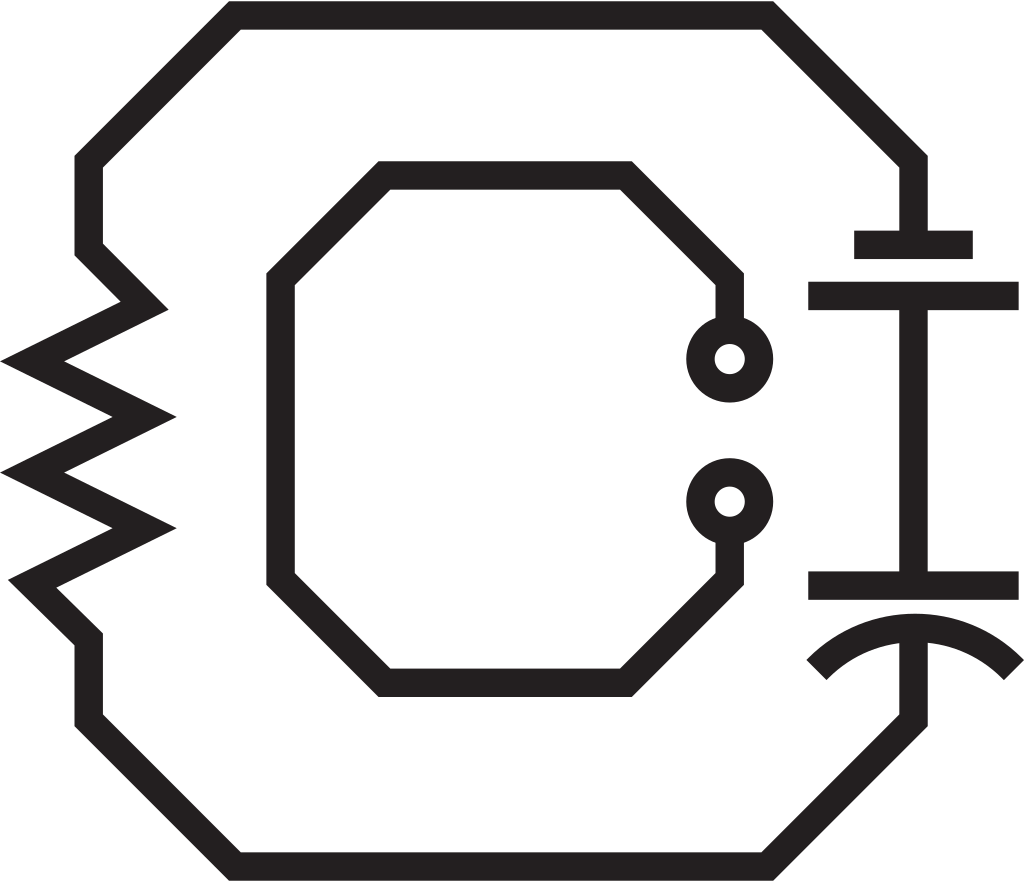
\includegraphics[height=0.635cm]{pictures/logo/c3i.png}%
    \hspace{0.25cm}%
    
\includegraphics[height=0.635cm]{pictures/logo/m1_alpha.pdf}\par
    \vspace{-0.3cm}%
    \textcolor{UDSgreenSolidarite}{%
        \noindent\rule{\textwidth}{1pt}%
    }%
}%

\defbeamertemplate*{footline}{mytheme}{%
    \leavevmode%
    \hbox{%
        \begin{beamercolorbox}%
            [wd=.33\paperwidth, ht=2.25ex, dp=1ex, center]{author in head/foot}%
            \usebeamerfont{author in head/foot}%
                \initials
        \end{beamercolorbox}%
        \begin{beamercolorbox}%
            [wd=.34\paperwidth, ht=2.25ex, dp=1ex, center]%
            {title in head/foot}%
            \usebeamerfont{title in head/foot}%
                \textbf{\inserttitle}%
        \end{beamercolorbox}%
    }%
    \begin{beamercolorbox}%
        [wd=.33\paperwidth, ht=2.25ex, dp=1ex, right]%
        {date in head/foot}%
        \hfill\usebeamerfont{date in head/foot}%
            \today{}%
        \hfill%
        \insertframenumber{} / \inserttotalframenumber%
        \hspace*{2ex}%
    \end{beamercolorbox}%
}%





% --------------- BUILD SETTINGS ----------------
\pdfcompresslevel=1
\pdfobjcompresslevel=1

% \tikzexternalize

% \dump
\csname endofdump\endcsname
\endofdump
%mylatex
